\documentclass[a4paper,10pt,oneside]{article}
\usepackage[polutonikogreek,italian]{babel}
\usepackage[utf8x]{inputenc}
\usepackage{amsmath}
\usepackage{amsthm}
\usepackage{amssymb}
\usepackage{amscd}
\usepackage{graphicx}
\usepackage{float}
\usepackage{array}
\usepackage{rotating}
\usepackage[small]{caption}
\usepackage{lscape}
\usepackage{fancybox}
\usepackage{booktabs}
\usepackage{subfigure}
\usepackage[noanswer]{exercise}
\parindent0ex
\renewcommand{\fboxsep}{0.4cm}
\usepackage{hyperref}
\renewcommand{\textfraction}{0.05}
\renewcommand{\topfraction}{0.95}
\renewcommand{\bottomfraction}{0.95}
\renewcommand{\floatpagefraction}{0.35}
\renewcommand{\ExerciseName}{Esercizio}
\renewcommand{\ExerciseListName}{Es}
\setcounter{totalnumber}{5}
\restylefloat{figure}
\begin{document}
\thispagestyle{empty}
 \section*{Moti parabolici}
\vspace{1cm}

In questa esperienza di laboratorio studieremo il moto bidimensionale di una pallina lanciata da un cannone ad elastico, analizzeremo sia il caso in cui la pallina ha una velocità iniziale parallela all'asse delle ascisse [\ref{fig:cannone2}] sia quello in cui la velocità forma un certo angolo $\theta$ con l'orizzontale [\ref{fig:cannone1}].
\begin{figure}[H]
 \subfigure[Lancio con vettore velocità iniziale formante un anglo $\theta$ con l'orizzontale]{
   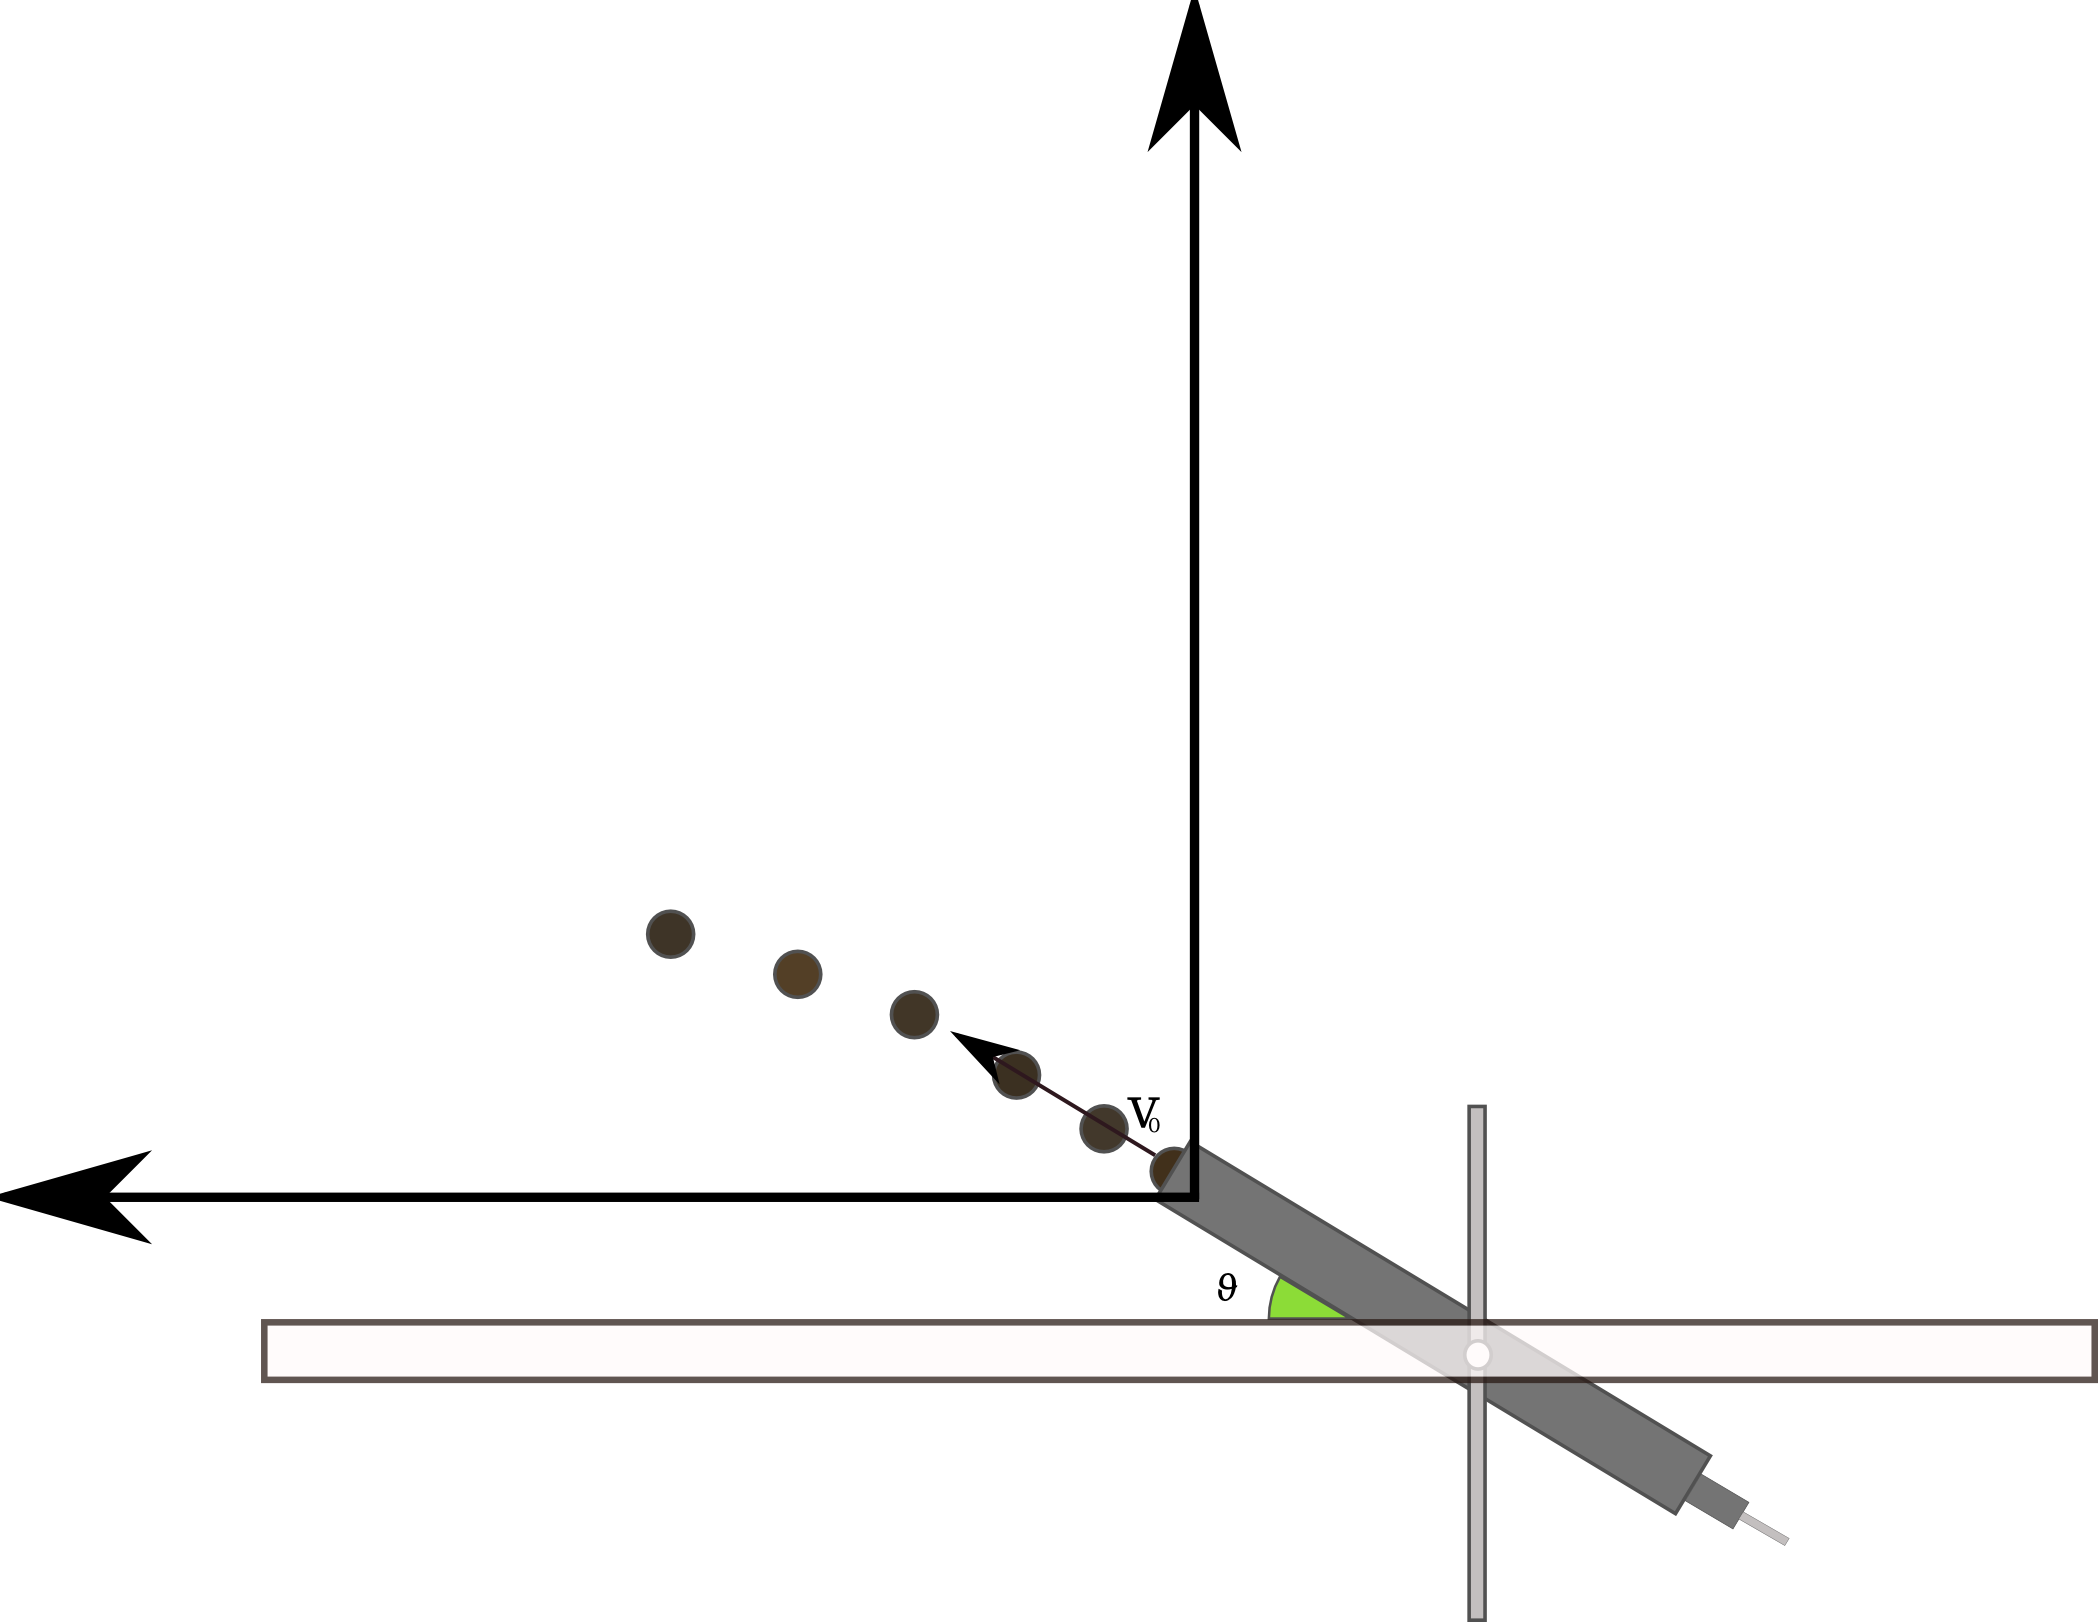
\includegraphics[width=0.5\textwidth]{./immagini/cannone1.png}
    \label{fig:cannone1}}
 \subfigure[Lancio con vettore velocità orizzontale]{
    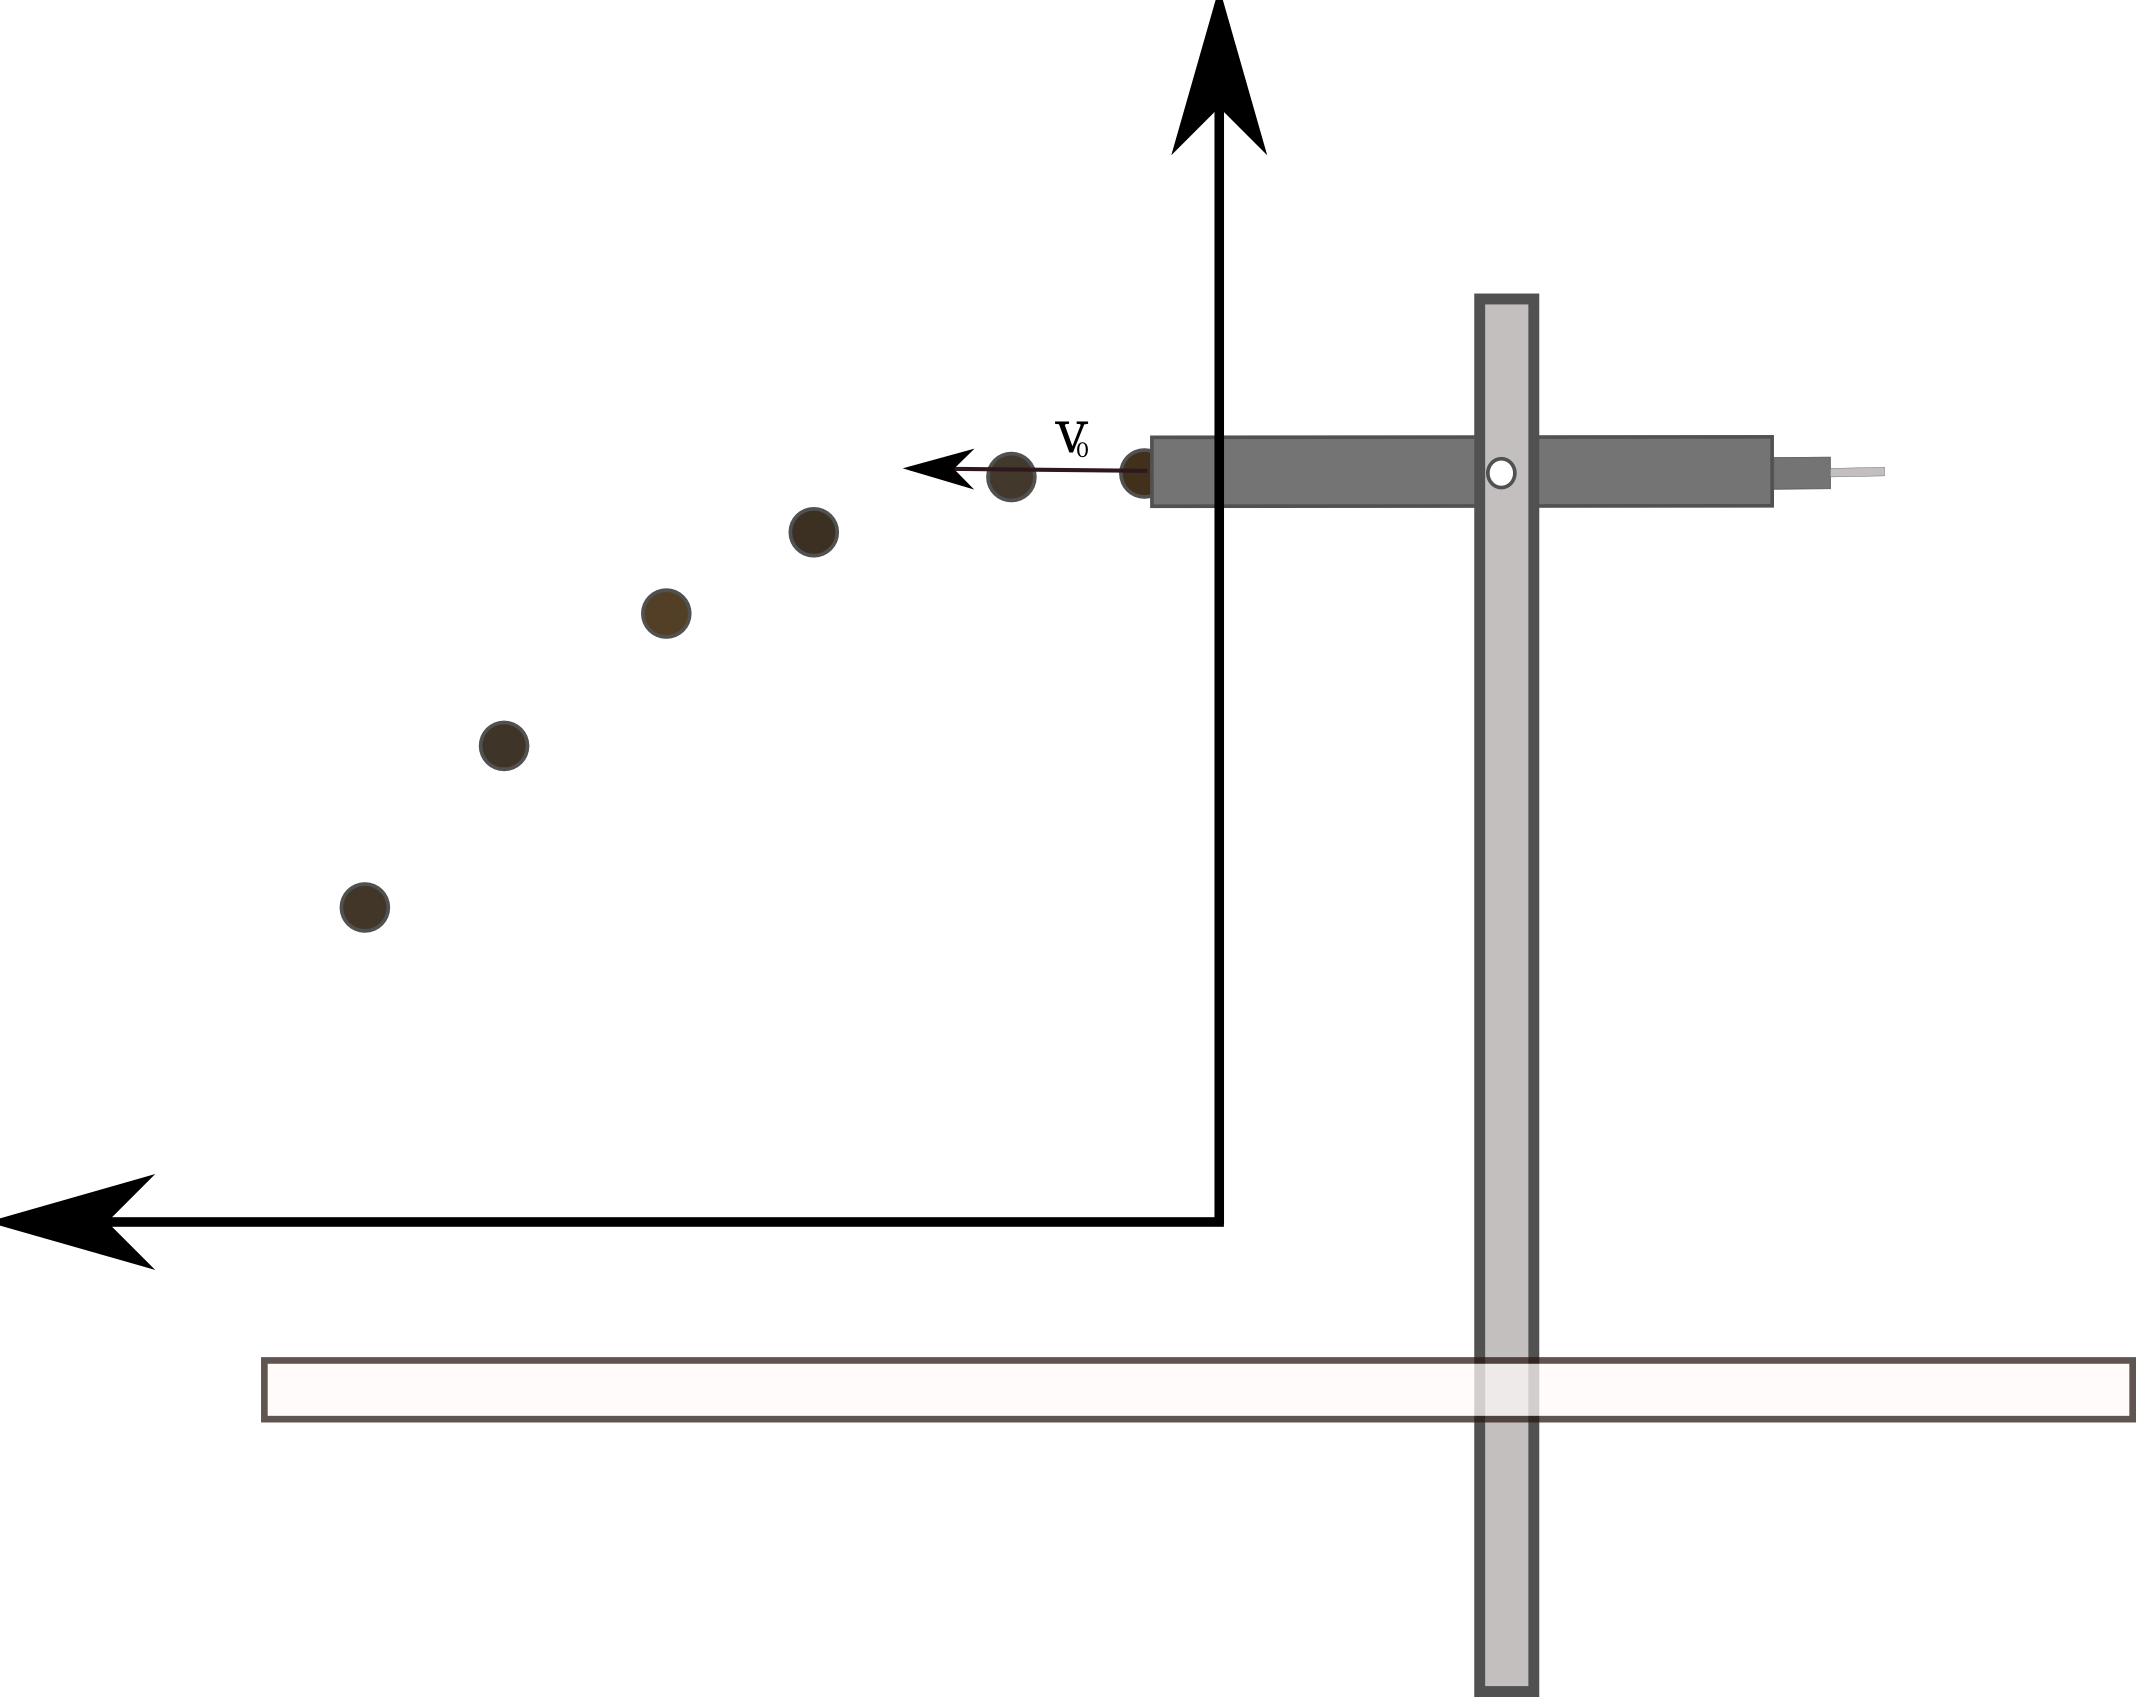
\includegraphics[width=0.5\textwidth]{./immagini/cannone2.png}
    \label{fig:cannone2}}
\caption{Lancio di una pallina con un cannone ad elastico}
\label{fig:sistema}
\end{figure}


\section*{Velocità iniziale parallela all'asse orizzontale}

Analizziamo matematicamente il problema: il punto materiale di cui dobbiamo studiare il moto possiede una velocità iniziale (nel momento in cui fuoriesce dalla bocca del cannone) parallela all'asse orizzontale possiamo quindi scrivere rispetto al sistema di riferimento di figura [\ref{fig:sistema}] :
\begin{equation}
 \mathbf{v}_0=(v_0,0)
\end{equation}
dove $v_0=|\mathbf{v}_0|$. Dopo essere fuoriuscita dal cannone alla quota $y_0$ la nostra pallina sarà animata da un moto accelerato lungo l'asse verticale e da un moto uniforme lungo l'asse orizzontale, il vettore velocità ad un istante di tempo successivo alla partenza risulta quindi:
\begin{equation}\label{eq:vel1}
 \mathbf{v}(t)=(v_0,-gt)
\end{equation}
analogamente a quanto fatto per i moti unidimensionali possiamo derivare il vettore posizione ad un tempo $t$ della nostra pallina:
\begin{equation}\label{eq:vel2}
 \mathbf{r}(t)=(v_0t,y_0-\frac{1}{2}gt^2)
\end{equation}
le equazioni [\ref{eq:vel1}] e [\ref{eq:vel2}] sono state scritte supponendo che i moti lungo i due assi siano indipendenti ovvero supponendo che la velocità della nostra pallina sia un vettore.
Girando un filmato ad alta frequenza del moto della pallina espulsa dal cannone (figura [\ref{fig:orizzontale_xy}]) è possibile ottenere una prova sperimentale dell'indipendenza del moto verticale da quello orizzontale. Dalla figura [\ref{fig:orizzontale_x}] notiamo come, a meno degli errori di misura, la distanza orizzontale tra due successive posizioni della pallina sia costante, dalla figura [\ref{fig:orizzontale_y}] deduciamo invece che lo spostamento verticale tra due posizioni successive della pallina è proporzionale al quadrato del tempo (moto uniformemente accelerato).

\begin{figure}[H]
 \subfigure[La pallina compie spostamenti orizzontali uguali in intervalli di tempo uguali, il moto è uniforme]{
  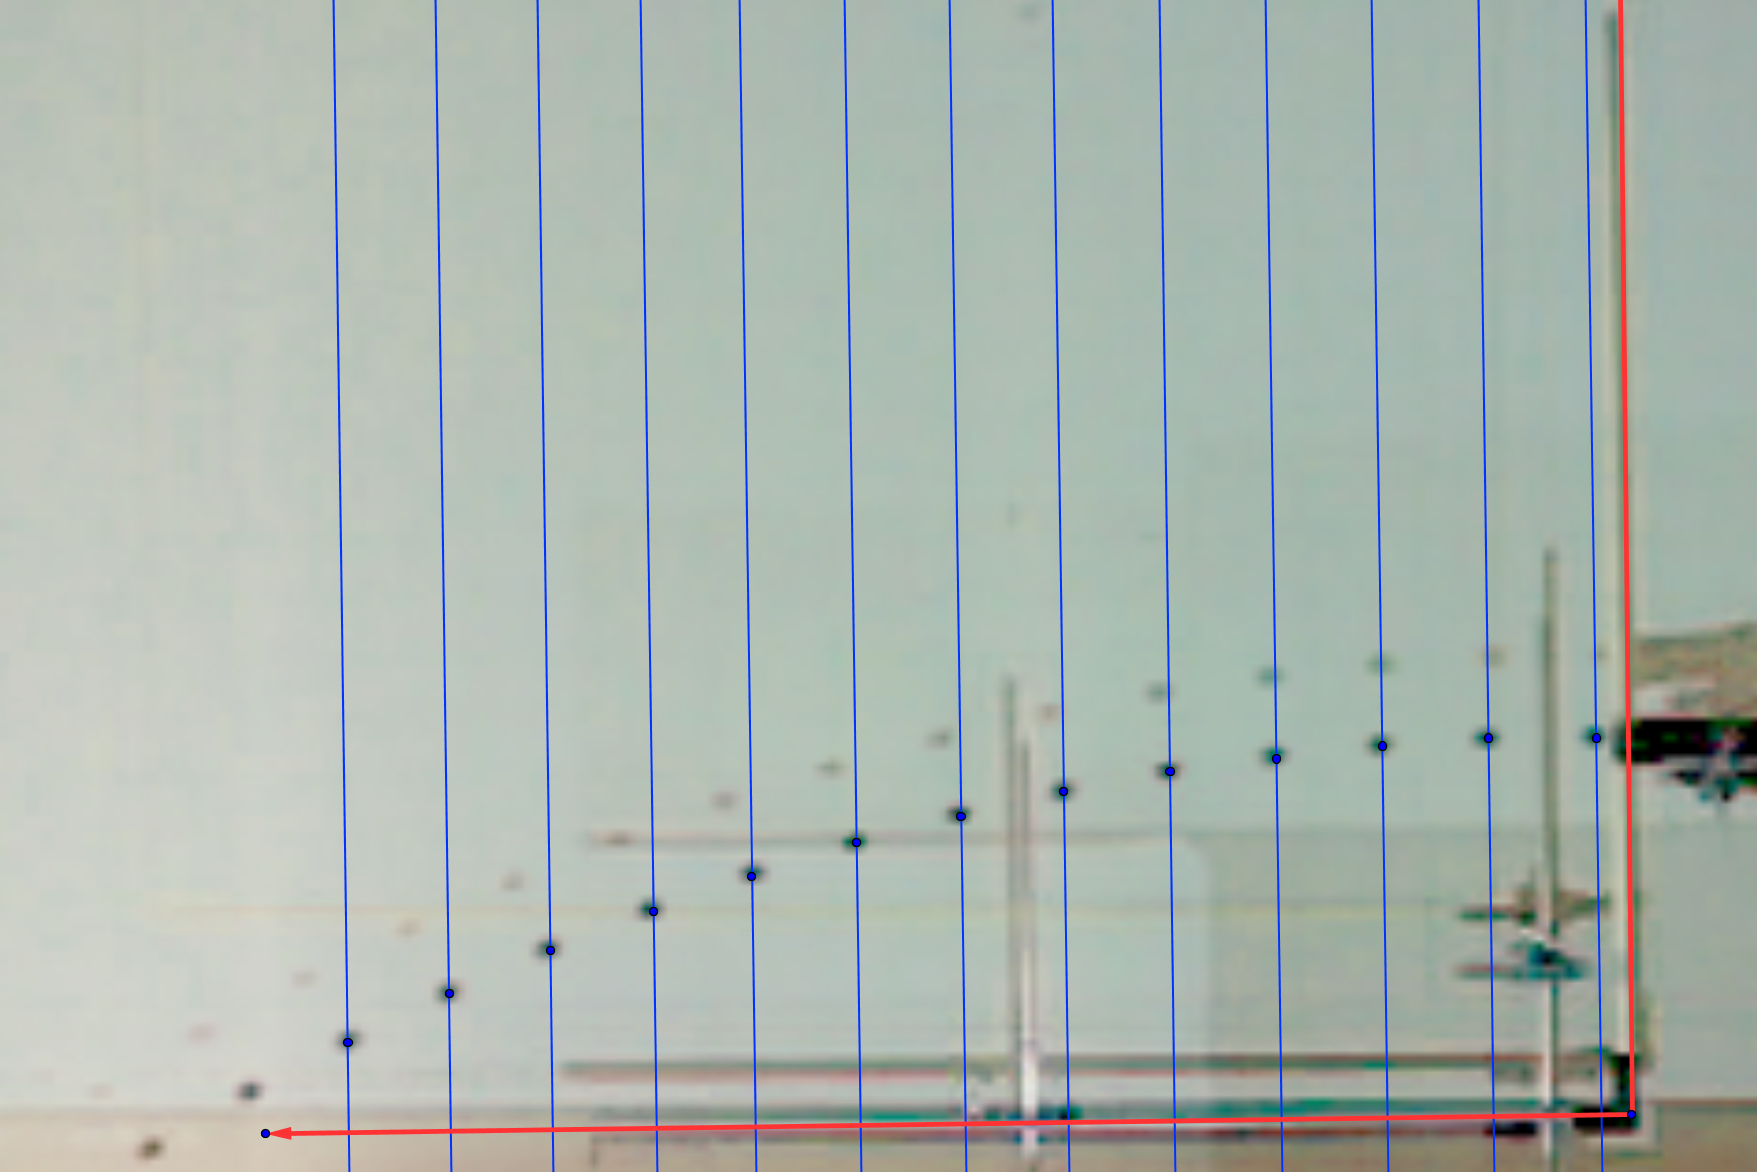
\includegraphics[width=0.5\textwidth]{./immagini/orizzontale_spaziamento_x.png}
  \label{fig:orizzontale_x}
 }
  \subfigure[La pallina compie spostamenti diversi in tempi uguali: il moto è accelerato]{
  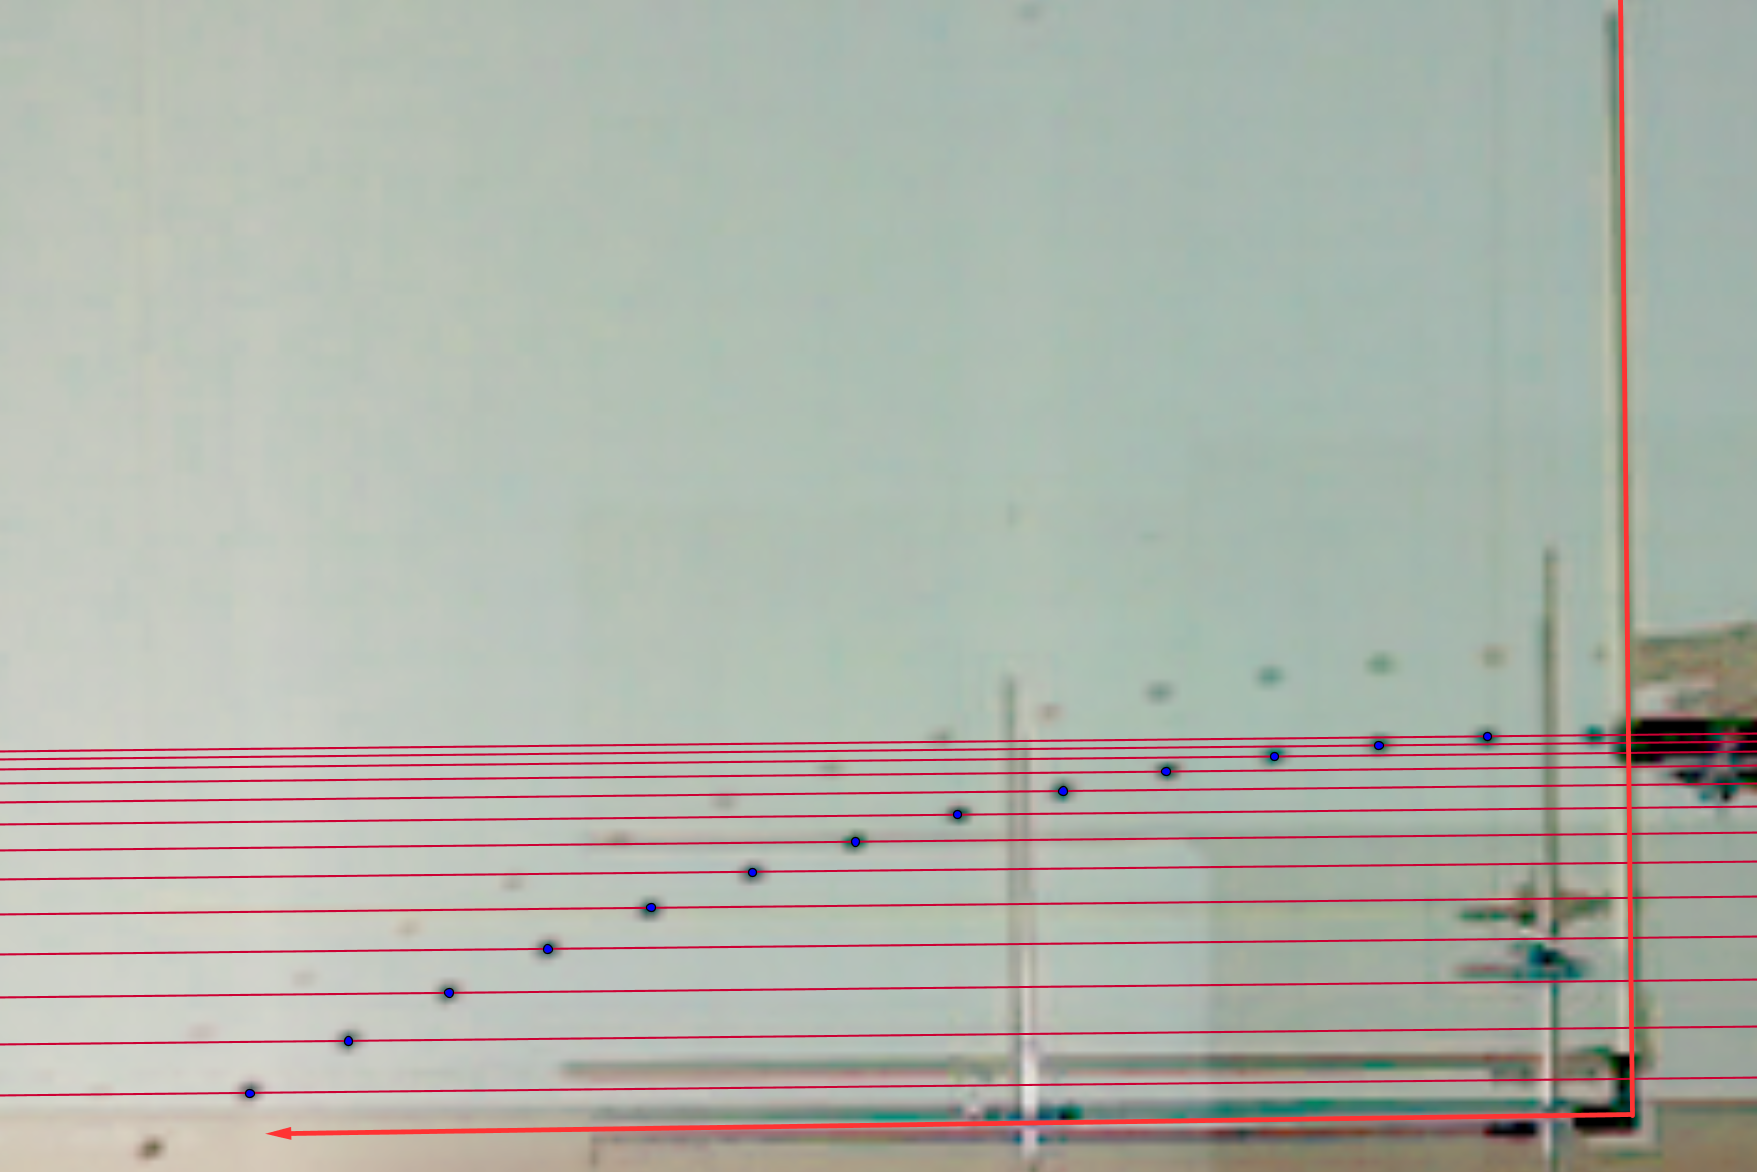
\includegraphics[width=0.5\textwidth]{./immagini/orizzontale_spaziamento_y.png}
    \label{fig:orizzontale_y}
  }
\caption{Il moto bidimensionale della pallina può essere scomposto in un moto uniforme orizzontale e in un moto uniformemente accelerato verticale}\label{fig:orizzontale_xy}
\end{figure}

\section*{Velocità iniziale formante un angolo $\theta$ con l'orizzontale}

Nel  caso più generale in cui la velocità iniziale della pallina forma un angolo $\theta$ con l'orizzontale l'analisi matematica del problema è leggermente più complessa rispetto a quanto esposto per la situazione particolare in cui $\theta=0$.
Per prima cosa calcoliamo le componenti della velocità all'istante zero di uscita dal cannone, detto $v_0$ il modulo della velocità possiamo scrivere:
\begin{equation}
 \mathbf{v}_0=(v_0\cos\theta,v_0\sin\theta)
\end{equation}
la velocità ad un tempo generico $t$ dopo il lancio diventa quindi:
\begin{equation}
 \mathbf{v}(t)=(v_0\cos\theta,v_0\sin\theta-gt)
\end{equation}
la componente orizzontale della velocità è costante esattamente come nel caso precedente, la componente verticale differisce dal caso con $\theta=0$ per la presenza di una componente verticale non nulla della velocità iniziale.
Utilizzando le conoscenze acquisite durante la trattazione dei moti unidimensionali possiamo scrivere per il vettore posizione:
\begin{equation}\label{eq:pos_incl}
 \mathbf{r}(t)=(v_0\cos\theta t,v_0\sin\theta t-\frac{1}{2}gt^2)
\end{equation}
notiamo ancora che la [\ref{eq:pos_incl}] è ottenuta considerando indipendenti il moto lungo l'asse orizzontale e quello lungo l'asse verticale.


Analizziamo ora le figure [\ref{fig:inclinato_x}] e [\ref{fig:inclinato_y}]. Per la prima possiamo ripetere quanto detto nel caso del moto con velocità iniziale parallela all'asse orizzontale. Soffermiamoci, quindi, sulla seconda figura e notiamo come su una singola parallela all'asse delle ascisse siano presenti due immagini della pallina: una nella fase ascendente ed una nella fase discendente. Questo dimostra come durante il moto di ascesa e quello di discesa, la pallina si trovi a quote uguali in tempi simmetrici rispetto all'istante in cui la quota è massima: se chiamiamo $t^*$ l'istante di tempo in cui la quota è massima negli istanti $t^*+\delta$ e $t^* -\delta$ con $\delta <t^*$ la quota è la medesima.


\begin{figure}[H]
 \subfigure[La pallina compie spostamenti orizzontali uguali in intervalli di tempo uguali, il moto è uniforme]{
  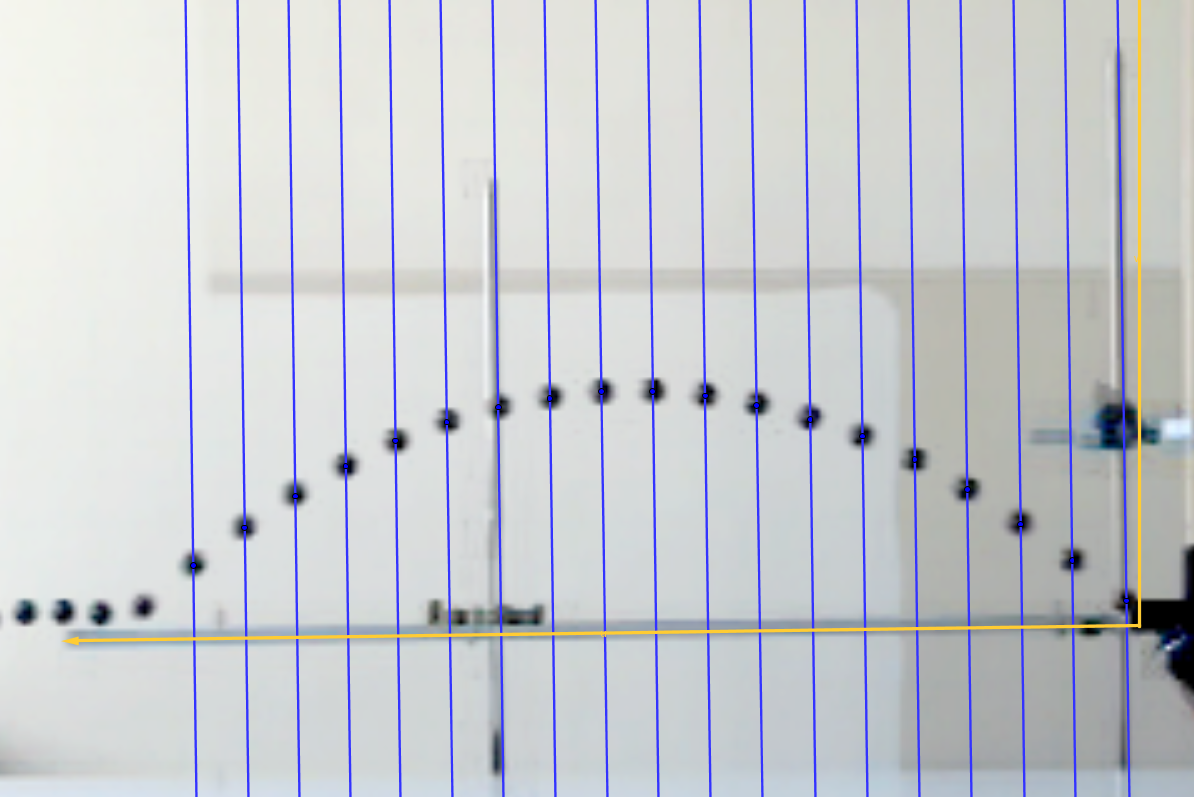
\includegraphics[width=0.5\textwidth]{./immagini/inclinato_intervalli_x.png}
  \label{fig:inclinato_x}
 }
  \subfigure[In istanti di tempo simmetrici a quello di massima elevazione la pallina si trova a quote uguali]{
  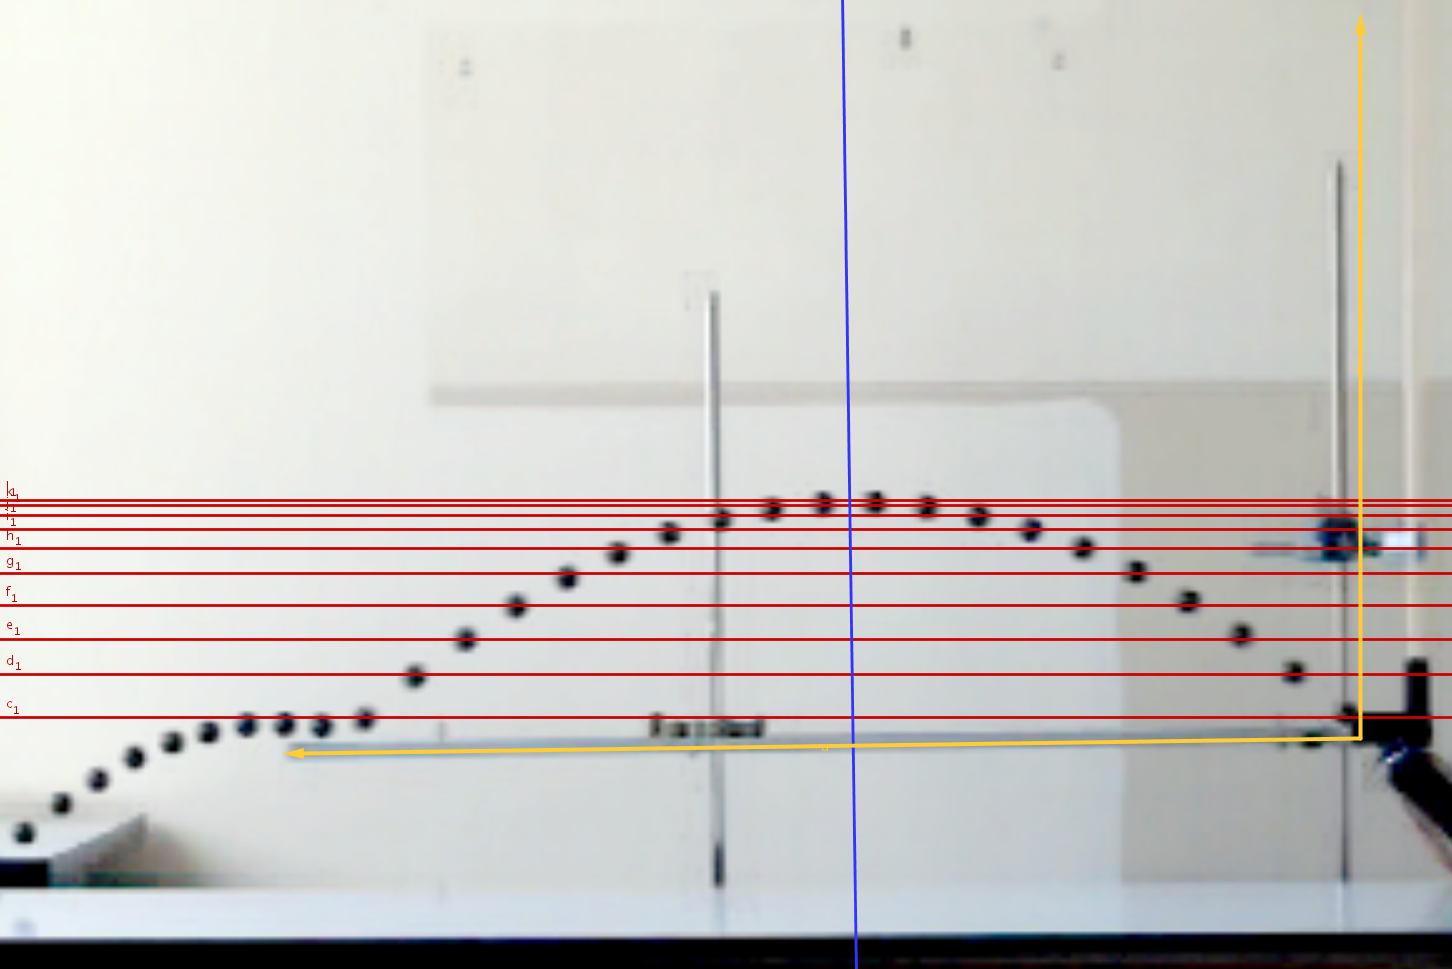
\includegraphics[width=0.5\textwidth]{./immagini/inclinato_intervalli_y.png}
    \label{fig:inclinato_y}
  }
\caption{Il moto bidimensionale della pallina può essere scomposto in un moto uniforme orizzontale e in un moto uniformemente accelerato verticale}\label{fig:inclinato_xy}
\end{figure}


\subsection*{Vettori spostamento, velocità media ed accelerazione media}

In figura [\ref{fig:posizione}] sono riportati i vettori $\mathbf{r}_{11}$ ed $\mathbf{r}_{14}$ relativi alla posizione 11 e alla posizione 14 della pallina lungo la sua traiettoria. Il vettore spostamento tra le posizioni indicate dai due vettori precedenti è definito come:
\begin{equation}
 \Delta \mathbf{s}=\mathbf{r}_{14}-\mathbf{r}_{11}
\end{equation}
ovvero come la variazione della posizione. Tramite il vettore spostamento possiamo definire il vettore velocità media in analogia a quanto fatto nel caso unidimensionale:
\begin{equation}\label{eq:v_media}
 \mathbf{v}_m=\frac{\Delta \mathbf{s}}{\Delta t}
\end{equation}
dalla [\ref{eq:v_media}] deduciamo che il vettore velocità media ha lo stesso verso e la stessa direzione del vettore spostamento.
Diversamente da quanto visto per la velocità media l'accelerazione istantanea non sarà collineare alla velocità media della pallina. Nel caso in esame, dato che il moto è uniformemente accelerato, possiamo scrivere il vettore accelerazione istantanea il quale avrà una componente orizzontale nulla, dato che in tale direzione la velocità è costante, ed una componente verticale pari all'accelerazione di gravità:
\begin{equation}\label{eq:accelerazione_inc}
 \mathbf{a}(t)=(0,-g)
\end{equation}


\begin{figure}[H]
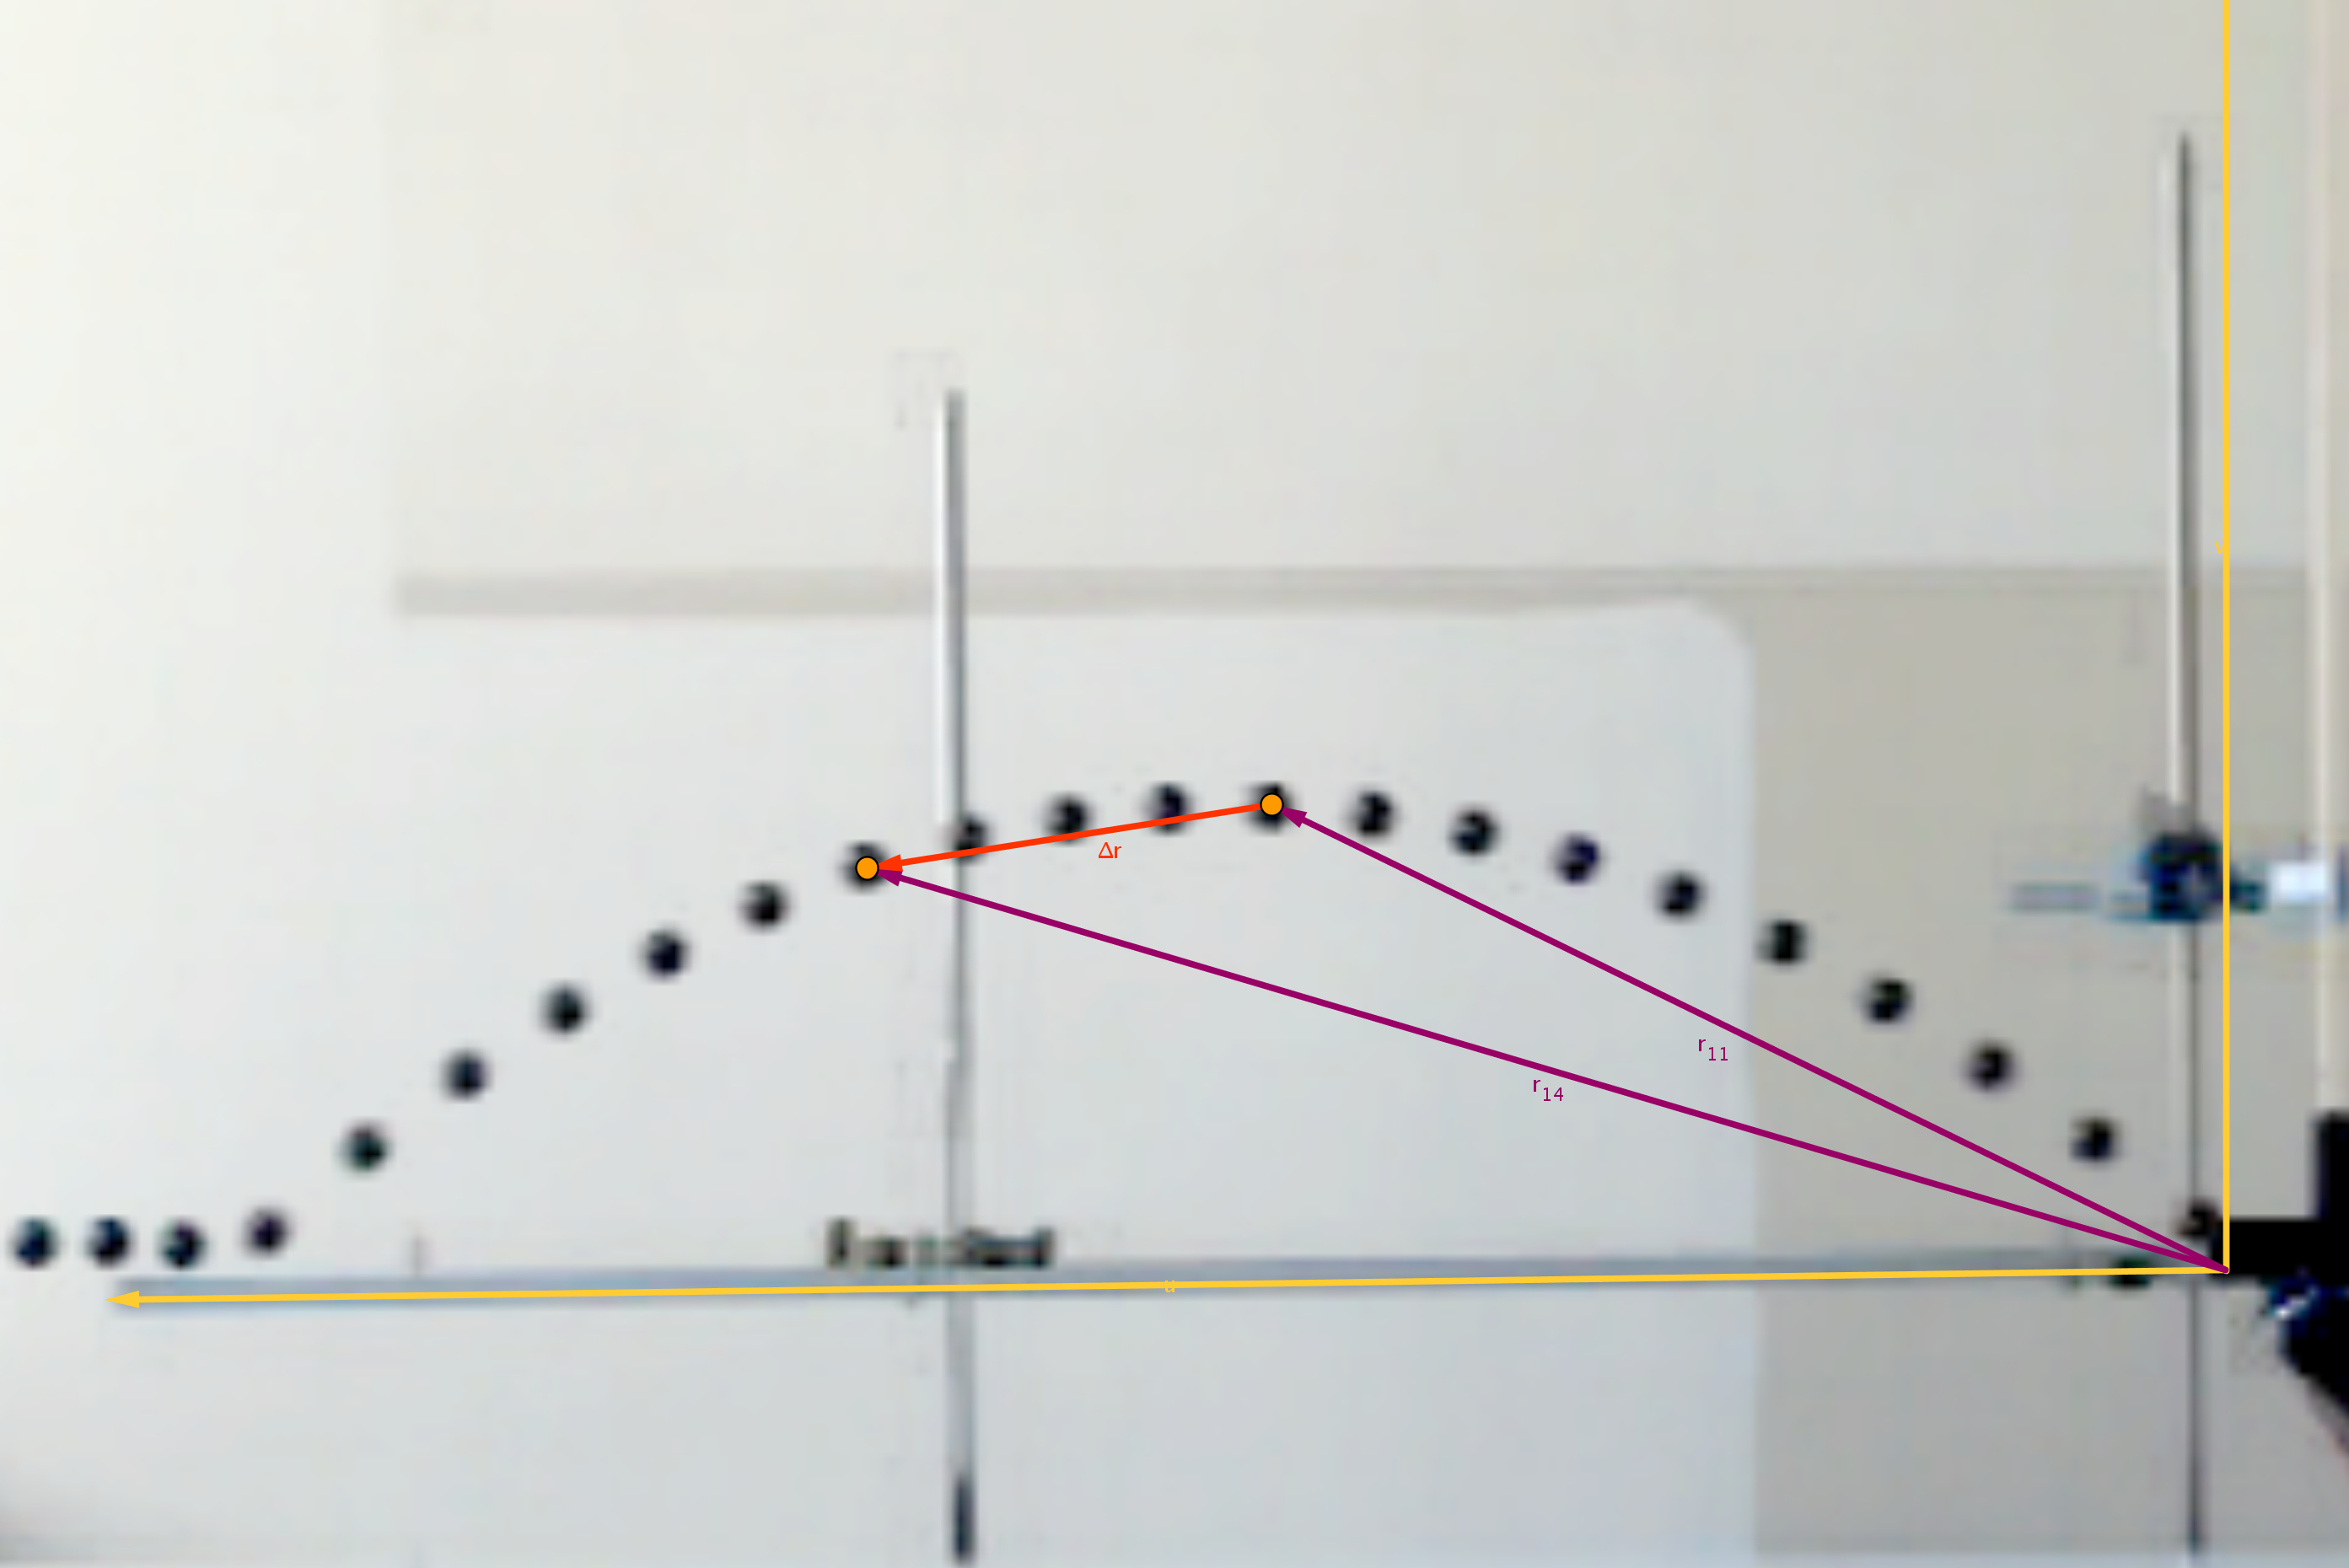
\includegraphics[width=\textwidth]{./immagini/vettori_posizione.png}
\caption{Il vettore posizione $\mathbf{r}$ della pallina in due istanti di tempo diversi. Notiamo come il piede di tale vettore si trovi nell'origine del sistema di coordinate e il vertice nel centro della pallina}\label{fig:posizione}
\end{figure}
Dalla [\ref{eq:accelerazione_inc}] si evince come in un moto bidimensionale accelerazione e velocità non sono in generale collineari.
Similmente a quanto fatto nel caso unidimensionale possiamo definire l'accelerazione media come il rapporto tra la variazione di velocità e l'intervallo di tempo in cui questa variazione avviene:
\begin{equation}
 \mathbf{a}_m=\frac{\Delta \mathbf{v}}{\Delta t}
\end{equation}
in figura [\ref{fig:a_media}] è riportato il vettore variazione di velocità per intervallo di tempo quadro $\Delta \mathbf{v}(\Delta t)^2$, è chiaramente visibile come questo non sia, in generale, diretto come il vettore velocità (media).
Il vettore accelerazione media non coinciderà con il vettore accelerazione istantanea ma ne sarà unicamente una approssimazione tanto più buona quanto più piccolo sarà l'intervallo di tempo $\Delta t $.

\begin{figure}[H]
 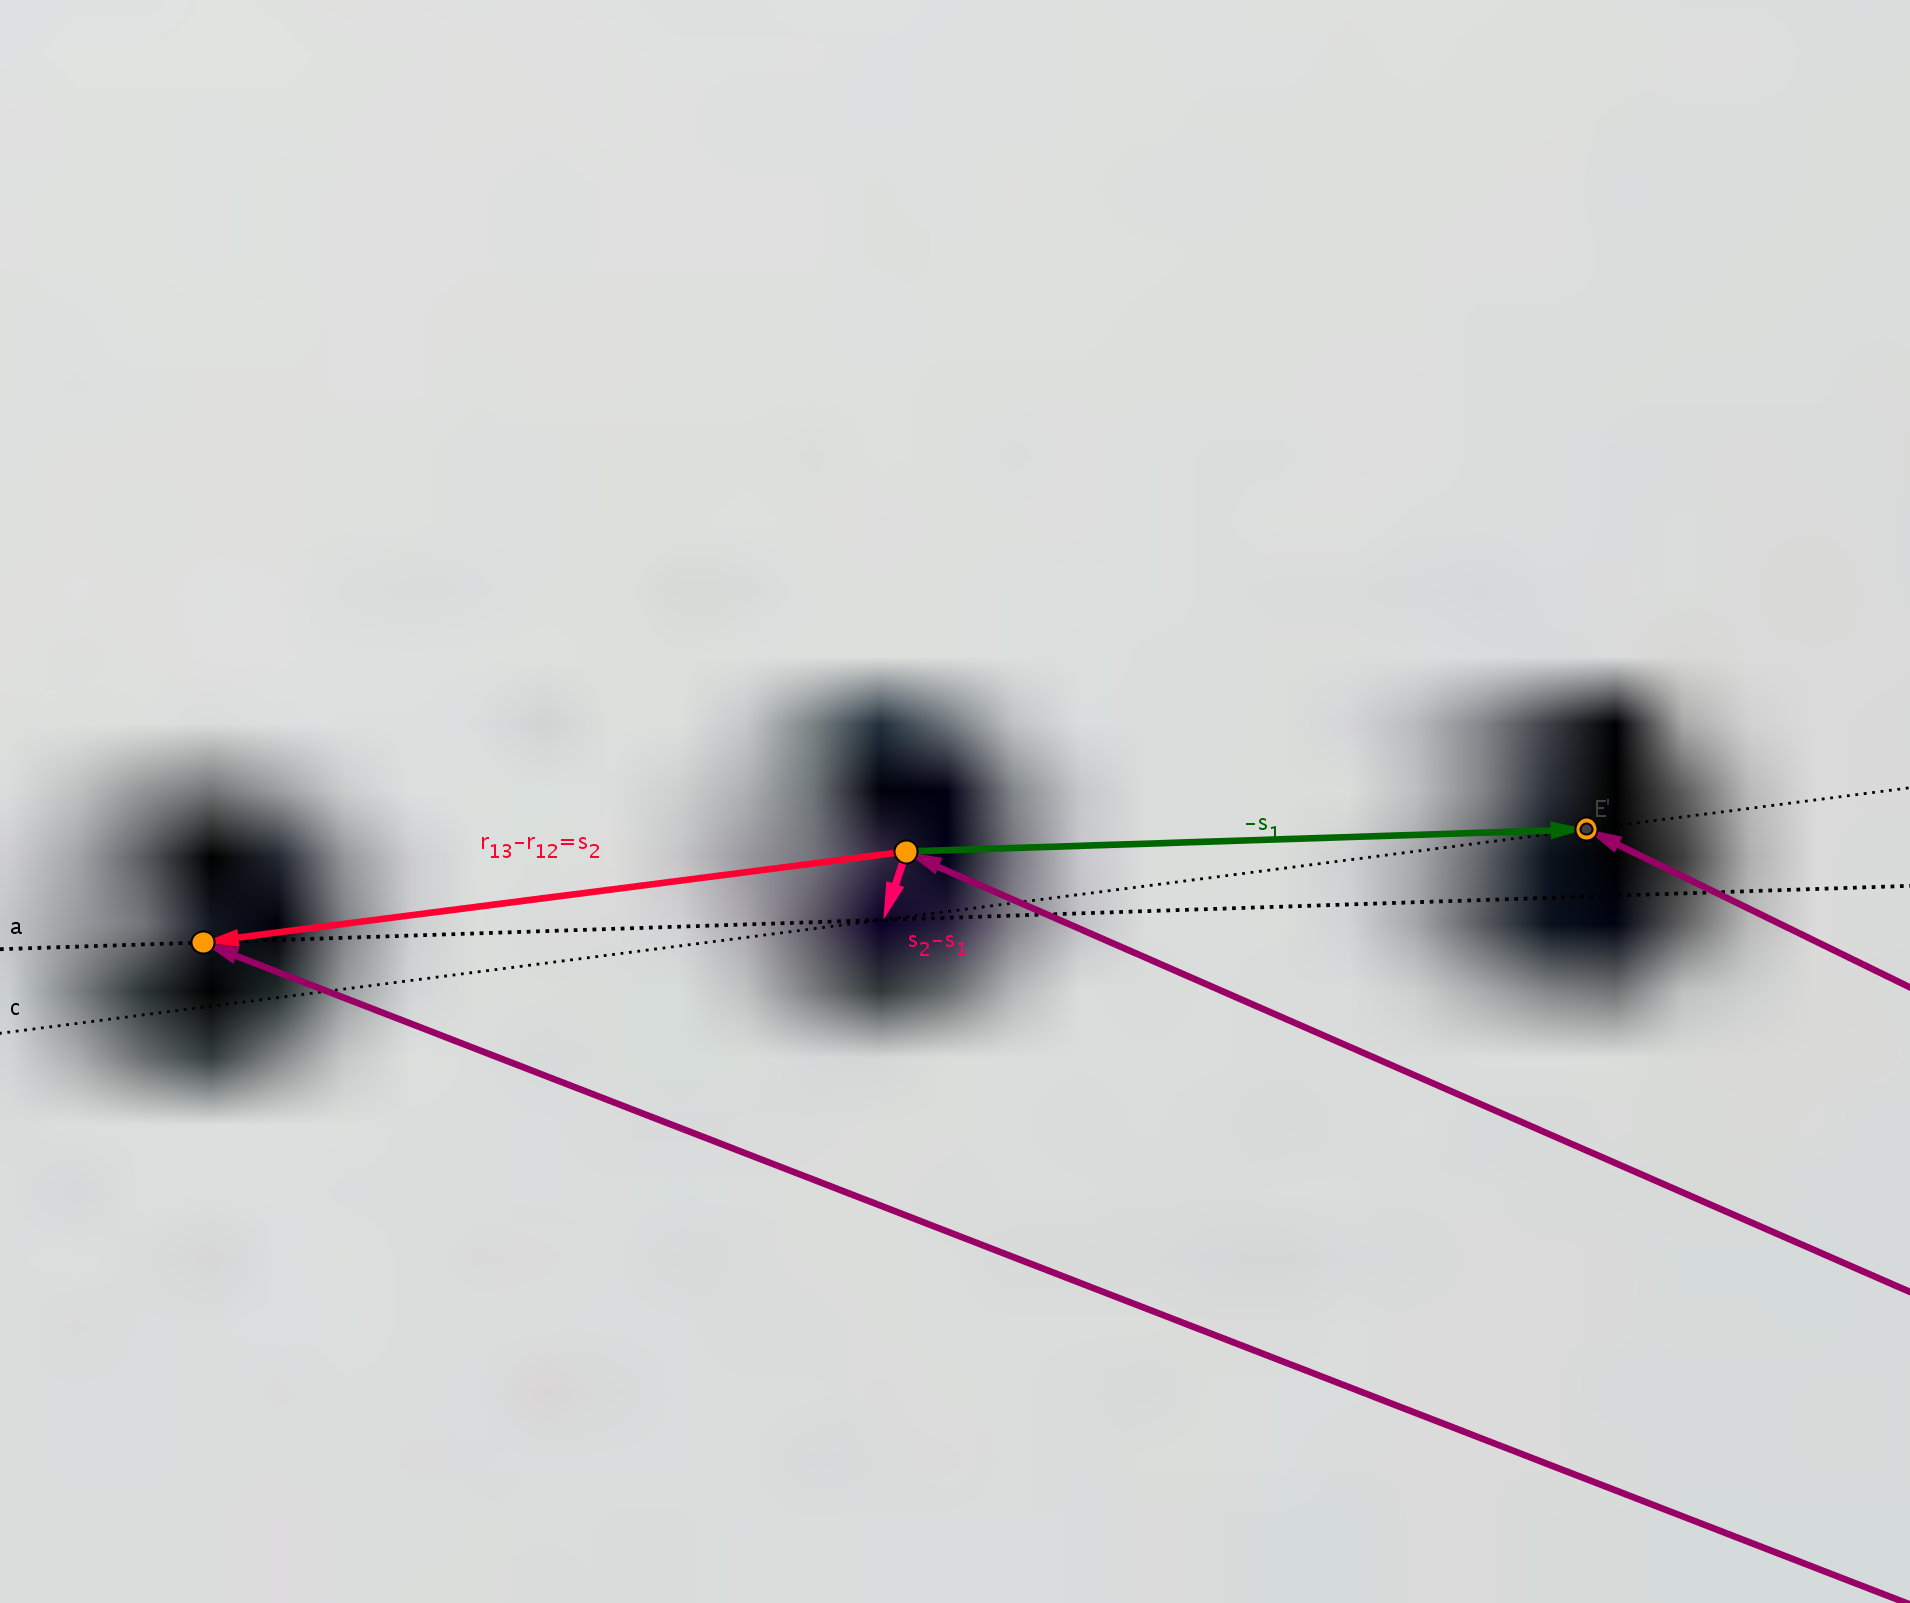
\includegraphics[width=\textwidth]{./immagini/vettori_variazione_velocita.png}
\caption{Il vettore $\mathbf{a}_m(\Delta t)^2$ collineare ed equiverso all'accelerazione media non è collineare alla velocità media}\label{fig:a_media}
\end{figure}

\subsection*{Traiettoria}

Conoscendo il vettore posizione $\mathbf{r}(t)$ possiamo ricavare la traiettoria della pallina soggetta ad un moto accelerato lungo l'asse verticale ed uno a velocità costante lungo l'asse orizzontale. Siccome le componenti del vettore posizione $\mathbf{r}$ espresse in coordinate cartesiane rappresentano le coordinate della pallina ad un certo istante di tempo $t$ possiamo scrivere il sistema:
\begin{equation}\label{eq:syst1}
\begin{cases}
x=v_0\cos\theta t\\
y=v_0\sin\theta t-\frac{1}{2}gt^2
\end{cases}
\end{equation}
Per ottenere l'equazione della traiettoria dobbiamo cercare una relazione indipendente dal tempo tra le variabili $x$ ed $y$. Dalla [\ref{eq:syst1}] vediamo che è sufficiente ricavare il tempo dalla prima equazione del sistema e sostituirlo nella seconda:
\begin{equation}
\begin{cases}
t=\dfrac{x}{v_0\cos\theta}\\
\\
y=v_0\sin\theta t-\frac{1}{2}gt^2
\end{cases}
\end{equation}
da cui ricaviamo:
\begin{equation}
 y=\tan\theta x-\dfrac{gx^2}{2v_0^2\cos^2\theta}
\end{equation}
ovvero l'equazione di una parabola con la concavità rivolta verso il basso.


\subsection*{Note}
Le figure riportate in questa breve dispensa sono state ottenute elaborando un filmato ad alta frequenza ripreso con una Casio Ex-fc150. Per la suddivisione del filmato in fotogrammi è stato usato \emph{ffmpeg} \url{www.ffmpeg.org} per la composizione delle immagini il programma \emph{Imagemagick} \url{www.imegemagick.org}, per disegnare vettori e linee sull'immagine si è utilizzato il programma \emph{Geogebra} \url{www.geogebra.org}. Immagini, filmati e file geogebra sono disponibili nella sezione laboratorio di \url{cartan.e-moka.net}


\end{document}